%************************************************
\chapter{Vectores}\label{ch:vectores}
%************************************************

El concepto de vector es básico para el estudio de funciones de varias variables, da una motivación
geométrica para todo lo que veremos. En esta sección trataremos algunas propiedades del vector
que necesitamos para las secciones siguientes. Una propiedad significativa de todos los enunciados 
siguientes es que aplican f\'acilmente para 2-dimensión, 3-dimensión y n-dimensión.

\section{Un punto en el espacio}

Sabemos que un número puede ser usado para representar un punto en una línea recta, siempre y cuando se
elija una unidad de longuitud.

Un par de números (un par ordenado) $(x,y)$ puede ser usado para representar un punto en un plano.

\begin{figure}[!ht]%
    \centering
    \subfloat[Punto en el plano]{{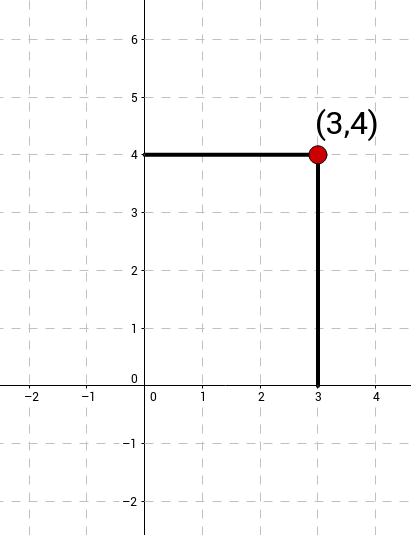
\includegraphics[width=0.35\textwidth]{gfx/punto-plano} }}%
    \qquad
    \subfloat[Punto en el espacio]{{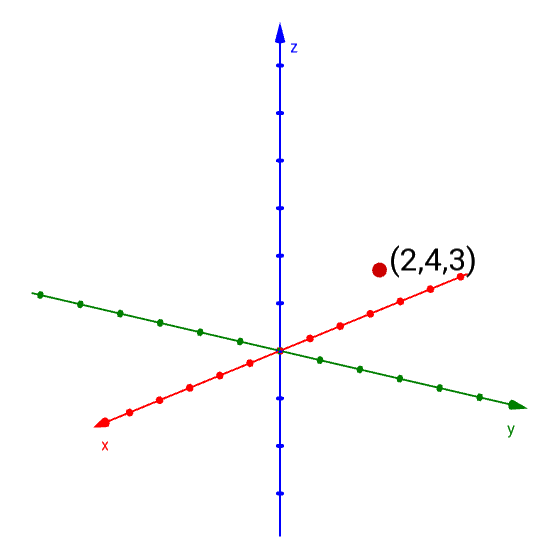
\includegraphics[width=0.5\textwidth]{gfx/punto-espacio} }}%
    \label{fig:example}%
\end{figure}

Ahora observemos que $(x,y,z)$ puede ser usado para representar un punto en el espacio, esto es un
punto en 3-dimensión, o 3-espacio. Simplemente agregamos un nuevo eje.

En vez de usar $x,y,z$ podemos usar $(x_{1},x_{2},x_{3})$. A la línea se le puede llamar 1-espacio y
al plano, naturalmente, 2-espacio.

Aunque no podemos dibujar un punto en 4-espacio, no hay nada que nos prevenga considerarlo, una cuarteta
de números

$$(x_{1},x_{2},x_{3},x_{4})$$

es un punto en 4-espacio. Una quinteta denotar\'ia un punto en 5-espacio, si continuamos llegamos a la siguiente
definición.

\begin{definition}
    Un punto en n-espacio es una n-tupla ordenado de números
    $$ (x_{1},x_{2}, \ldots ,x_{n}) $$
    con $n$ un entero positivo.
\end{definition}

La mayor\'ia de nuestros ejemplos serán para los casos $n=2$, $n=3$. Así podremos visualizarlos f\'acilmente a
lo largo de este texto. Pero nuestras definiciones y demostraciones comunmente serán para el n-espacio y así
cubrir ambos casos. Cabe mencionar que el caso $n=4$ ocurre en Física, por ejemplo, la idea de tomar al tiempo
como cuarta coordenada es vieja. Ya desde la \emph{Encyclopédie} de Diderot, en el siglo XVIII, d'Alembert escribe 
en su artículo sobre dimensión:

\vspace{0.5cm}

\emph{La manera de considerar cantidades con m\'as de tres dimensiones es tan natural como los otros casos,
porque las letras algebraicas siempre pueden ser vistas como representación de números, ya sean racionales
o no. Antes mencion\'e que no era posible imaginarse mas de tres dimensiones. Un caballero astuto de quien soy
íntimo cree lo contrario, que podr\'ia tomarse a la duración como la cuarta dimensión. Esta idea puede ser
discutida, pero para mí, tiene su mérito por el solo hecho de ser nueva.}

\begin{flushright}
    \emph{Encyplopédie, Vol.4 (1754), p. 1010}
\end{flushright}

Observe como d'Alembert se refiere a un \emph{caballero astuto} cuando al parecer se refiere a s\'i mismo. El procede
con cautela al proponer una idea avanzada para su tiempo, la cual se hizo mas común en el siglo XX.

No nos queda de otra que definir como sumar puntos.

\begin{definition}
    Si $A$ y $B$ son puntos en n-espacio. $A=(a_{1},a_{2},\ldots,a_{n})$ y $B=(b_{1},b_{2},\ldots,b_{n})$. Entonces $A+B$
    se define
    $$ A + B = (a_{1} + b_{1}, a_{2} + b_{2}, \ldots, a_{n} + b_{n}) $$
\end{definition}

\begin{myExample}
    En el plano, si $A=(1,2)$ y $B=(-3,5)$, entonces
    $$ A + B = (-2,7) $$
\end{myExample}

\begin{myExample}
    En el espacio, si $A=(-1,\pi,3)$ y $B=(\sqrt{2},7,-2)$, entonces
    $$ A + B = (\sqrt{2} - 1, \pi + 7, 1) $$
\end{myExample}

\begin{definition}
    Si $c$ es cualquier número, entonces
    $$ cA = (ca_{1},\ldots,ca_{n}) $$
\end{definition}

\begin{myExample}
    Sea $A=(1,2)$ y $c=3$. Entonces
    $$cA = (3,6)$$
\end{myExample}

\begin{figure}[!ht]%
    \centering
    \subfloat[Punto en el plano]{{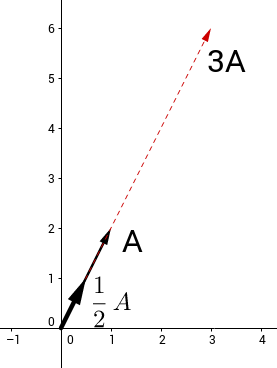
\includegraphics[width=0.45\textwidth]{gfx/producto-escalar} }}%
    \qquad
    \subfloat[Punto en el espacio]{{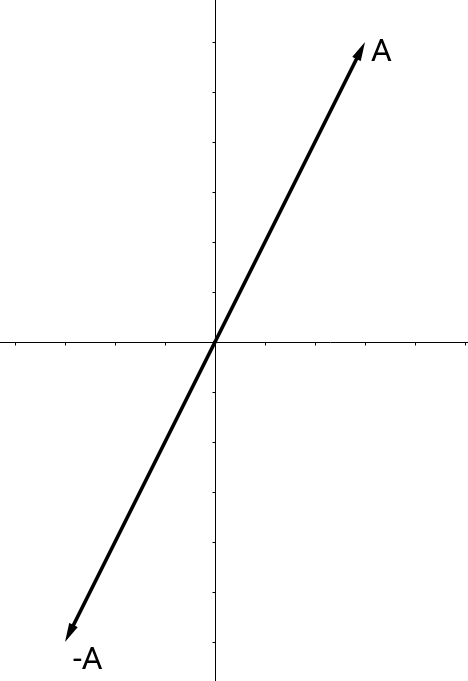
\includegraphics[width=0.45\textwidth]{gfx/producto-escalar2} }}%
    \label{fig:example}%
\end{figure}


Observe que multiplicar el vector $A$ por $3$ equivale a \emph{estirar} el vector $3$ veces, de igual forma
si $c=\frac{1}{2}$ entonces $cA$ ser\'ia la mitad de $A$. Si $c=-1$ entonces $cA$ tiene la misma \emph{magnitud}
que $A$ pero en sentido contrario.

\section{Vector localizado}

\begin{definition}
    Un vector localizado es un par ordenado de puntos $A$ y $B$, donde $A$ es el punto inicial y $B$ es el punto final. Se
    denota $\myVector{AB}$.
\end{definition}

Podemos obsvervar que en el plano,
$$ b_{1} = a_{1} + (b_{1} - a_{1}) $$
De forma similar,
$$ b_{2} = a_{2} + (b_{2} - a_{2}) $$

Cuando el punto inicial es el origen y el punto final es cualquier otro punto $A$ denotaremos al vector simplemente como $A$.

\section{Producto punto}

Daremos por entendido que a lo largo de esta sección seleccionaremos vectores que vivan en la misma dimensión.

\begin{definition}
    Sean $A$ y $B$ dos vectores en n-espacio. El producto punto
    $$ A \cdot B = a_{1}b_{1} + \ldots + a_{n}b_{n} $$
    Este producto es un número.
\end{definition}

\begin{myExample}
    Si $A=(1,3,-2)$ y $B=(-1,4,-3)$, entonces
    $$ A \cdot B = -1 + 12 + 6 = 17 $$
\end{myExample}

Veamos ahora unas propiedades básicas de este producto.

\begin{labeling}{}
    \item [\textbf{SP 1.}] Tenemos que $A \cdot B = B \cdot A$.
    \item [\textbf{SP 2.}] Si $A$,$B$,$C$ son tres vectores, entonces
        $$ A \cdot (B+C) = A \cdot B + A \cdot C = (B+C) \cdot A$$
    \item [\textbf{SP 3.}] Si $x$ es un número, entonces
        $$ (xA) \cdot B = x(A \cdot B) \quad \text{and} \quad A \cdot (xB) = x(A \cdot B) $$ 
    \item [\textbf{SP 4.}] Si $A=0$ es el \emph{vector cero}, entonces $A \cdot A = 0$, de lo contrario
        $$ A \cdot A > 0 $$
\end{labeling}

Algo de extrema importancia para este texto es el concepto de perpendicularidad entre vectores, a partir
de esto definiremos, en capítulos posteriores, lo que es un vector tangente.

\begin{definition}
    Sean $A$ y $B$ dos vectores. $A$ y $B$ son \emph{perpendiculares} (ortogonales) si
    $$ A \cdot B = 0 $$
\end{definition}

\section{La norma de un vector}

Una pregunta natural al estudiar vectores es ¿qué longuitud (magnitud) tienen?. Veremos a continuación
la definición de \emph{norma} de un vector, la cual contesta a nuestra pregunta.

\begin{definition}
    La norma de un vector $A$ es el número,
    $$ \| A \| = \sqrt{A \cdot A} $$
    Como $A \cdot A \ge 0$ podemos sacarle raíz cuadrada. 
\end{definition}

A la norma también se le conoce como \emph{magnitud} de A. Cuando $n=2$ y $A = (a,b)$, entonces
    $$ \| A \| = \sqrt{a^{2} + b^{2}} $$

Observe que para cualquier vector $A$ tenemos que 
$$ \| A \| = \| -A \| $$

\begin{definition}
    Sean $A$ y $B$ dos puntos cualquiera. La distancia entra $A$ y $B$ se define como
    $$ \| A - B \| = \sqrt{(A-B) \cdot (A-B)} $$
\end{definition}

\begin{myExample}\label{ex:distance}
    Sea $A = (-1,2)$ y $B = (3,4)$. Entonces la longuitud del vector $\myVector{AB}$ es $\|B-A\|$. Pero
    $B-A = (4,2)$. Entonces
    $$\|B-A\| = \sqrt{16+4} = \sqrt{20} $$
\end{myExample}

Sea $P$ un punto en el plano, y sea $a$ un número $> 0$. El conjunto de puntos $X$ tales que
$$ \| X - P \| < a $$
es llamado \emph{disco abierto} de radio $a$ y centro en $P$. Si en cambio
$$ \| X - P \| \le a $$
el conjunto es llamado \emph{disco cerrado} de radio $a$ y centro en $P$. El conjunto de puntos
$X$ tales que
$$ \| X - P \| = a $$
es llamado \emph{circurferencia} de radio $a$ y centro en $P$.

Si transladamos P al espacio tridimensional, los conjuntos anteriores son llamados \emph{bola abierta},
\emph{bola cerrada} y \emph{esfera} respectivamente.

\section{De cuaterniones a vectores}
Los vectores como los conocemos nacieron en las primeras dos decadas del siglo IXX con la representación
geométrica de los números complejos. En 1837, William Rowan Hamilton (1805-1865) mostró que los números
complejos pod\'ian ser considerados abstractamente como pares ordenados $(a,b)$ de números reales. Esta idea
era parte de una investigación para encontrar una forma de representar "números" de dos dimensiones en tres
dimensiones, nadie logró hacerlo preservando las propiedades básicas de los reales y complejos. \\

\begin{figure}[!ht]
  \begin{center}
    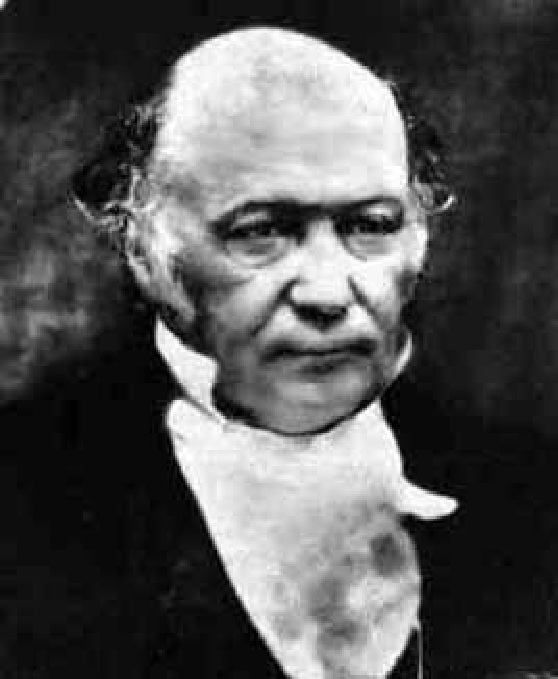
\includegraphics[width=0.3\textwidth]{gfx/hamilton}
  \end{center}
  \caption{Hamilton}
\end{figure}

Después de mucha frustración, Hamilton dejó su busqueda del tal sistema númerico de tres dimensiones e inventó
uno de cuatro dimensiones, lo llamó cuaterniones. Los cuaterniones de Hamilton se denotaban $q = w + ix + jy + kz$, donde, $w$,$x$,$y$ y $z$ eran números reales.

Aunque los cuaterniones fueron fuertemente aceptados por varios científicos, entre ellos Maxwell y Lord Kelvin,
ten\'ian un problema que incomodaba a los matemáticos. El producto de cuaterniones no es conmutativo ni homog\'eneo
, es decir, $pq = -qp$.

En el tiempo que Hamilton descubrió los cuaterniones, Hermann Grassmann (1809-1867) estaba escribiendo
"The Calculus of Extension (1844)", mejor conocido por su título en alemán, Ausdehnungslehre. En 1832
Grassmann comenzó el desarrollo de un nuevo cálculo geométrico y subsecuentemente usó este estudio para
simplificar porciones de dos trabajos clásicos, Analytical Mechanics de Joseph Louis Lagrange y Celestial
Mechanics de Pierre Simon Laplace. En su libro, Grassmann expande por primera vez la idea del concepto
de un vector (como $ix + jy + kz$ de los cuaterniones) de dos a tres y $n$ dimensiones, lo cual expandió
la idea de dimensión de un espacio.

\begin{figure}[!ht]
  \begin{center}
    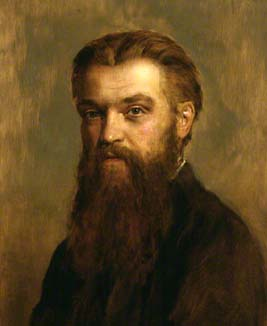
\includegraphics[width=0.3\textwidth]{gfx/clifford}
  \end{center}
  \caption{Clifford}
\end{figure}

William Kingdon Clifford (1845 - 1879) expresó profunda admiración por la obra de Grassmann, y claramente
favoreció a los vectores sobre los cuaterniones. Clifford separó el producto de dos cuaterniones en dos
productos diferentes de vectores, los cuales llamó producto escalar y producto vectorial, solucionando
el problema del producto de cuaterniones.

El desarrolo del álgebra de vectores y análisis vectorial como lo conocemos hoy día fue descrito en un conjunto
de notas por el matemático J. Williard Gibbs (1839-1903) para sus estudiantes de la Universidad de Yale.

%*****************************************
%*****************************************
%*****************************************
%*****************************************
%*****************************************




